109. \begin{figure}[ht!]
\center{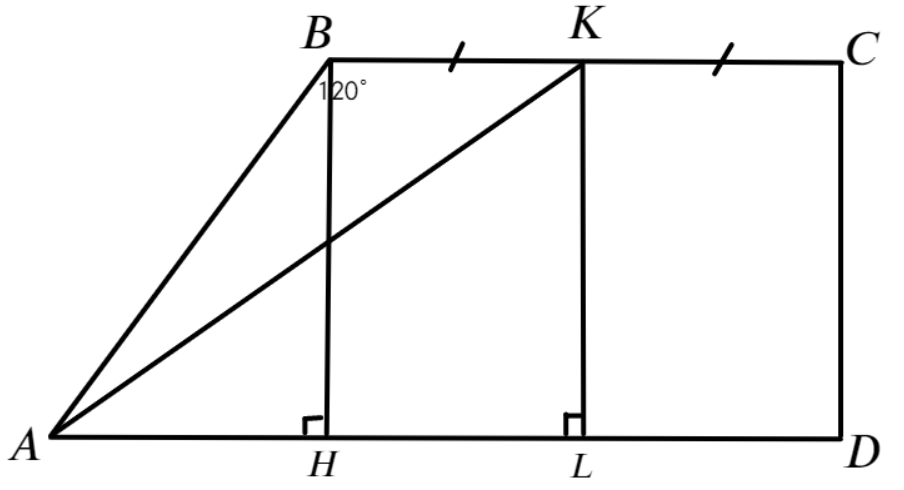
\includegraphics[scale=0.35]{g8-109.png}}
\end{figure}\\
Найдём $\angle A=180^\circ-120^\circ=60^\circ.$ Опустим перпендикуляры $KL$ и $BH,$ тогда $\angle ABH=90^\circ-60^\circ=30^\circ,$ поэтому $AH=\cfrac{1}{2}AB=\cfrac{1}{2}\cdot4=2,\ BH=KL=\sqrt{4^2-2^2}=2\sqrt{3}.$ В треугольнике $AKL:\ AL=AH+HL=2+2=4,$ тогда $AK=\sqrt{4^2+(2\sqrt{3})^2}=2\sqrt{7}$ по теореме Пифагора.\\
